\subsection{\label{subsecSHM}Comparison to statistical hadronization models}

The measured abundances of hadrons produced in heavy-ion collisions have been successfully described by statistical hadronization models over a wide range of energies~\cite{Andronic:2011yq,Cleymans:1998fq,Andronic:2005yp}. Statistical model calculations for central ultra-relativistic heavy-ion collisions are typically carried out in the grand-canonical ensemble. However, a grand-canonical description of particle production is only applicable if the volume $V=R^{3}$ of the system is sufficiently large and as a rule of thumb one needs $VT^{3} > 1$ for a grand-canonical description to hold~\cite{Hagedorn:1984uy,Rafelski:1980gk}. This condition must be fulfilled for each conserved charge separately.
Several attempts were made to extend the picture of statistical hadronization to smaller systems such as pp or even e$^{+}$e$^{-}$ collisions~\cite{Redlich:2009xx,Becattini:1996gy,Kraus:2008fh}. While particle ratios of non-strange particles are observed to be similar in small and large systems, the relative production of strange particles appears to be significantly lower in smaller systems. The data presented in~\cite{Adam:2016emw} show for the first time that there is a continuous increase of strangeness production with increasing event multiplicity across various collision systems. In the strangeness canonical approach, it is assumed that the total amount of strange hadrons in the volume is small with respect to non-strange hadrons. Thus the conservation of strangeness is guaranteed locally and not only globally while the bulk of the particles is still described in the grand-canonical ensemble. For further details on this approach, we refer for instance to~\cite{BraunMunzinger:2003zd,Hamieh:2000tk,Cleymans:2004bf}. The study presented here utilizes the implementation in the THERMUS 3.0 code~\cite{Wheaton:2004qb}. Alternative implementations of the statistical model are for instance adopted in the codes of the GSI-Heidelberg~\cite{Andronic:2005yp,Andronic:2017pug} and SHARE~\cite{PETRAN20142056} groups.

%The experimental data is taken from~\cite{Adam:2016emw,Abelev:2013haa,Adam:2016bpr,Adam:2015vsf,Abelev:2014uua,Abelev:2013xaa,Abelev:2013vea,ABELEV:2013zaa}.

\subsubsection{Correlation volume for strangeness production} 

Previous studies based on THERMUS were targeted to describe the evolution of multi-strange particle production in p-Pb collisions as a function of event multiplicity~\cite{Adam:2015vsf}. In this case, the volume for particle production was chosen such that the charged pion multiplicity d$N_{\pi}$/d$y$ at midrapidity corresponding to a window of $y = \pm 0.5$ units was correctly described by the model. This approach is equivalent to calculating strangeness suppression for a  system whose total extension only corresponds to one unit of rapidity. Consequently, the model describes qualitatively the suppression pattern, but overestimates the reduction of strangeness at small multiplicities. The discrepancy increases even further if this approach is extended to the smaller multiplicities which are covered in pp collisions.


\begin{figure*}[t!]
  \begin{flushleft}
    \center{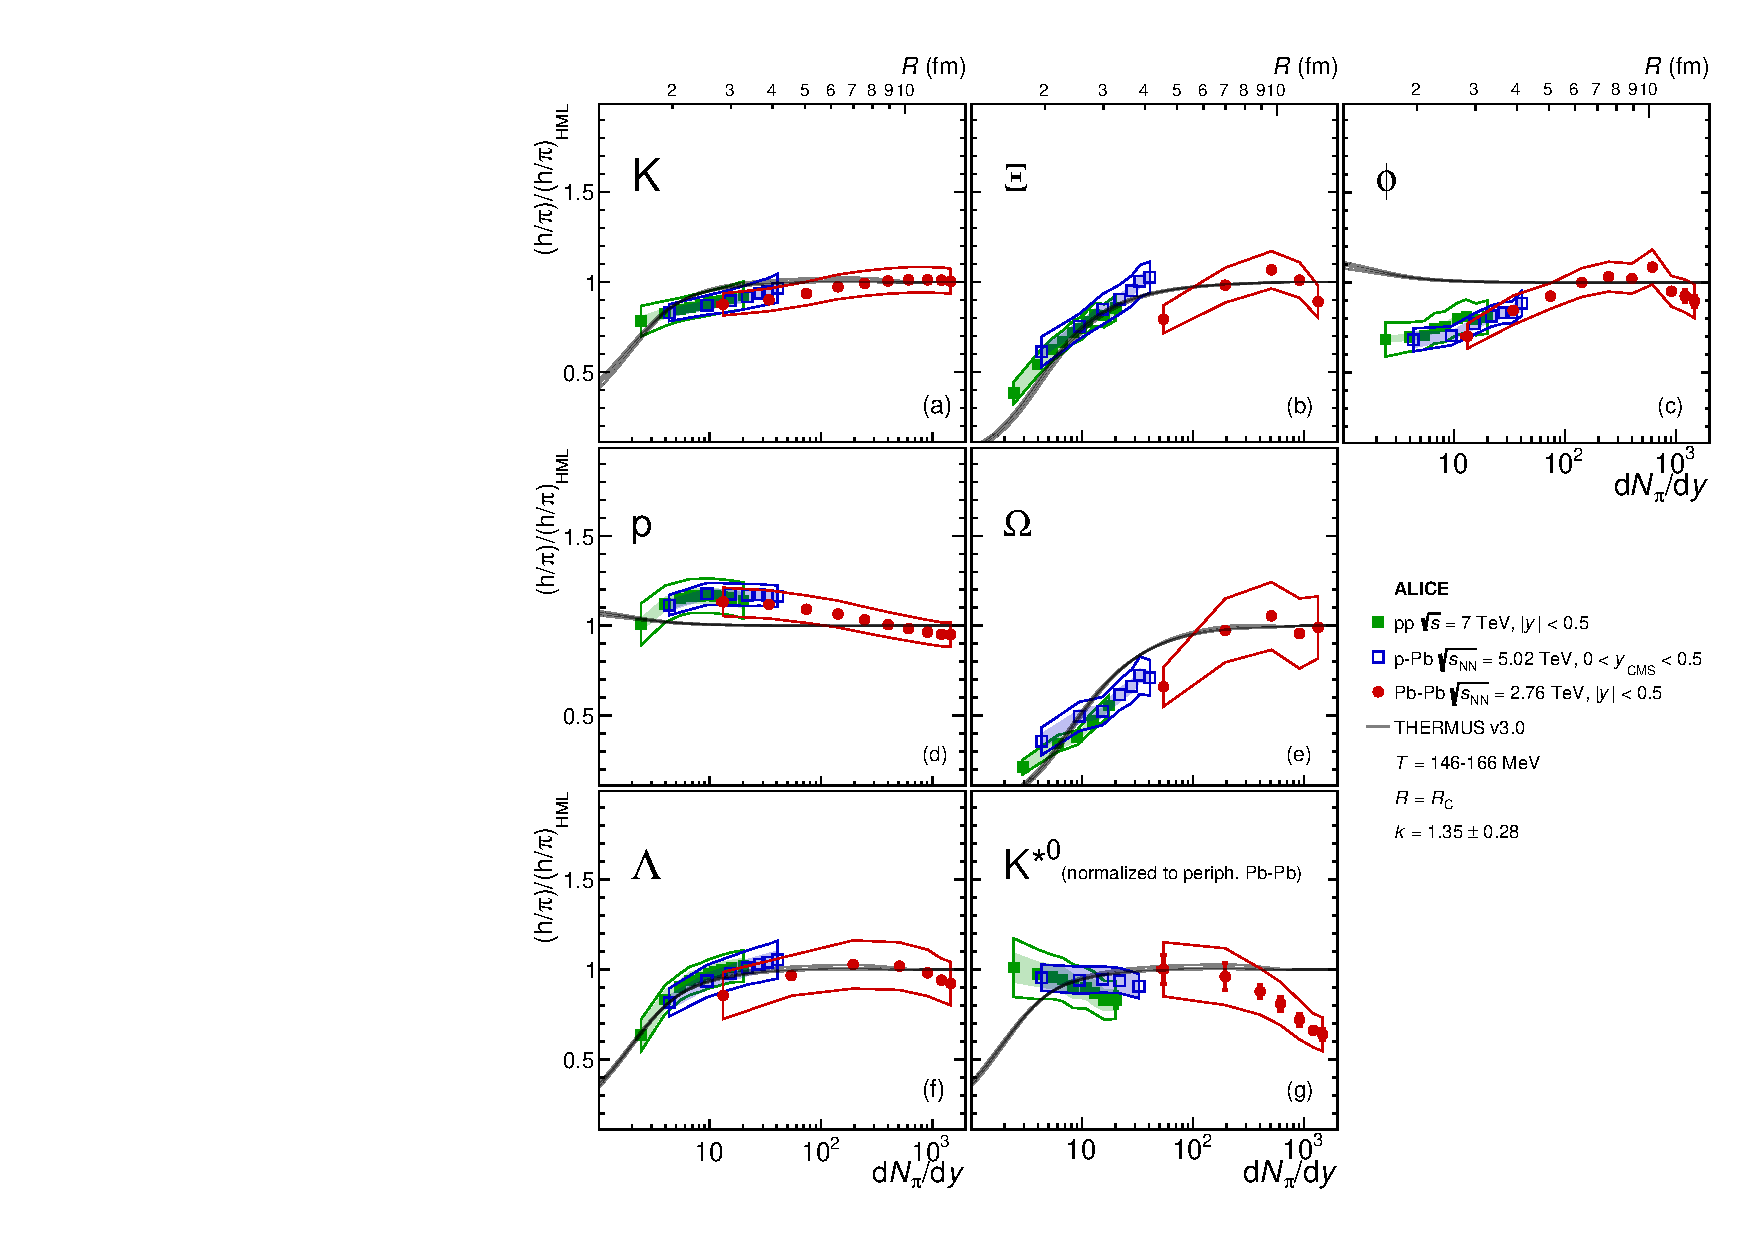
\includegraphics[width=\textwidth]{figures/Discussion_SHM_Suppression.pdf}}
    \end{flushleft}
    \caption{Ratios of the production yields to pions for several particle species as a function of the midrapidity pion yields for pp, \pPb\ and \PbPb\ colliding systems compared to the THERMUS model prediction for the strangeness canonical suppression (continuous curves), in which only the system size is varied.  All values except for the \kstar\ are normalized to the high multiplicity limit (see text for details). The upper axis shows the radius $R$ of the correlation volume $V=R^{3}$ which corresponds to the predicted particle ratios. The variations in model prediction curves correspond to variations of the chemical freeze-out temperature between 146, 156 and 166~MeV. Reference p-Pb and Pb-Pb data from \cite{Abelev:2013haa, Adam:2015vsf, 2016720, Abelev:2013xaa,2014196}.
    %The data is taken from~\cite{Adam:2016emw,Abelev:2013haa,Adam:2016bpr,Adam:2015vsf,Abelev:2014uua,Abelev:2013xaa,Abelev:2013vea,ABELEV:2013zaa}.
    }
    \label{fig:SHM_Suppression}
\end{figure*}  


In the study presented here, a similar approach as in~\cite{Adam:2015vsf} is followed: the strangeness saturation parameter is fixed to $\gamma_S = 1$, the chemical potentials associated to baryon and electric charge quantum numbers are set to zero. The chemical freeze-out temperature $T_{ch}$ is varied from 146 to 166~MeV as in~\cite{Adam:2015vsf} following recent results from  Lattice QCD calculations and their uncertainties~\cite{Bazavov:2014pvz} as well as by fits to experimental data from central Pb-Pb collisions~\cite{Acharya:2017bso,Andronic:2017pug}. Ratios of the production yields to pions are investigated for several particle species. In order to cancel the influence of the freeze-out temperature and to isolate the volume dependence, all ratios except for \kstar\ are normalized to the high multiplicity limit, i.e. the grand-canonical saturation value for the model and the mean ratio in the 0-60\% most central Pb-Pb collisions for the data.
As the production rates of short-lived resonances in central heavy-ion collisions might be reduced by re-scattering effects in the hadronic phase~\cite{Abelev:2014uua,Adam:2016bpr}, the values for K$^{0*}$ were normalized to the most peripheral bin in Pb-Pb collisions. The resulting double ratios are shown in Fig.~\ref{fig:SHM_Suppression}.

In contrast to~\cite{Adam:2015vsf}, the total volume $V$ of the fireball was determined differently. While the strangeness conservation volume is also imposed to be of the size of the fireball ($V=V_C$), its absolute magnitude is not fixed to reproduce the pion multiplicity in a window of $y = \pm 0.5$ at midrapidity. Instead, it is fixed to reproduce a pion multiplicity which is larger by a factor $k$ and thus corresponds to a larger rapidity window assuming a flat dependence of particle production as a function of rapidity. The same factor $k$ was used for all particles and multiplicities. In practice, $k$ corresponds to a constant scaling factor of d$N_{\pi}$/d$y$ (the x-axis in Fig.~\ref{fig:SHM_Suppression}), and this feature is used for its numerical determination: the exact value of $k$ was optimized in a one-parameter fit of the functions describing the evolution of the double ratios versus d$N_{\pi}$/d$y$ to the experimental data.  For the determination of the systematic uncertainty on the value of $k$, an alternative normalization scheme for the data was applied (normalization to the highest available centrality bin) and the procedure for the determination of $k$ was repeated. A value of $k=1.35 \pm 0.28$ is obtained corresponding to a rapidity window of $y = \pm 0.67$. The results thus indicate that the total correlation volume for strangeness production extends over about 1.35 units in rapidity. In other words, strangeness as a conserved quantity in QCD can be effectively equilibrated over this distance in the system. Similar values can be obtained from purely theoretical considerations on causality constraints~\cite{Castorina:2013mba}. Furthermore, the size of the correlation window is also compatible with similar estimates for charm production~\cite{Andronic:2003zv,Andronic:2006ky}. We also note that this value is smaller than the plateau in the rapidity distribution at LHC energies which extends typically over three to four units~\cite{Adam:2015gka,Abbas:2013bpa} and is thus meaningful from a physical point of view.
 

\subsubsection{Comparison to experimental data} 

As shown in Fig.~\ref{fig:SHM_Suppression} this approach allows for a qualitative description of particle ratios as a function of event multiplicity. They can be naturally described within the framework of strangeness canonical suppression. The deviations observed for the \kstar\ meson in central Pb-Pb collisions can be ascribed to the aforementioned re-scattering effects in the hadronic phase~\cite{Knospe:2015nva}. Furthermore, differences between the model and the data in the most peripheral Pb-Pb collisions in case of $\Omega$ and $\Xi$ can be potentially reduced with core-corona corrections~\cite{Aichelin:2008mi}. 
 
 
From a quantitative point of view, essentially all data points can be described within 1-2 standard deviations. A potentially different trend is only observed for the $\phi$-meson for which -- as a strangeness-neutral particle -- a flat dependence as a function of event multiplicity is expected from the model, but which shows a rising and falling trend in data. Future experimental data will be needed in order to clarify the significance of this deviation. It must be noted, though, that the $\phi$-meson also deviates from a common blast-wave fit to other light-flavor hadrons in peripheral Pb-Pb collisions indicating an out-of-equilibrium production except for most central Pb-Pb collisions~\cite{Abelev:2014uua}.

Independently of the experimental precision and possible higher order effects in the particle production mechanisms, we find that the strangeness canonical approach can reproduce the multiplicity dependence of all measured 
light-flavor hadrons across various collision systems to within 10-20\%.



